
\subsection*{1.}

\paragraph{a.} L'aire du rectangle est \( x y = 49 \), d'où \( y = \dfrac{49}{x} \), puisque \( x \neq 0 \).

Le périmètre du rectangle est :
\[
p(x) = 2(x + y) = 2\left(x + \dfrac{49}{x}\right).
\]

\paragraph{b.} On a donc :
\[
p(10) = 2\left(10 + \dfrac{49}{10}\right) = 2(10 + 4{,}9) = 2 \times 14{,}9 = 29{,}8.
\]
On a \(p(x) = 2x + 2 \times \dfrac{49}{x} = 2x + \dfrac{98}{x} = f(x)\).

\subsection*{2.}

On dérive \(f\) comme somme de fonctions dérivables :
\[
f'(x) = 2 - \dfrac{98}{x^2} = \dfrac{2x^2 - 98}{x^2}.
\]

\subsection*{3.}

Comme \(x > 0 \Rightarrow x^2 > 0\), on déduit que le signe de \(f'(x)\) est celui de son numérateur.

\begin{align*}
&2x^2 - 98 > 0 \\
\iff &2(x^2 - 49) > 0 \\
\iff &x^2 - 49 > 0 \\
\iff &(x - 7)(x + 7) > 0.
\end{align*}
Le trinôme \(x^2 - 49\) est positif sauf sur l'intervalle \(\,] - 7 \,;\, 7 [\,\).

On en déduit que la fonction \(f\) est décroissante sur \(\,] 0 \,;\, 7 [\,\), puis croissante sur \(\,] 7 \,;\, +\infty [\,\), avec un minimum en :
\[
f(7) = 2 \times 7 + \dfrac{49}{7} = 14 + 7 = 21.
\]

\begin{center}
\begin{tikzpicture}
\tkzTabInit[lgt=3.5, espcl=4]{$x$ / 1, {Signe de $f'(x)$} / 1, {$f(x)$} / 2}{${0}$, ${7}$, ${+\infty}$}
\tkzTabLine{,-,0,+,}
\tkzTabVar{+/{$$},-/{$21$},+/{$$}}{/}
\end{tikzpicture}
\end{center}

\subsection*{4.}

Si \(x = 7\), alors \(y = \dfrac{49}{7} = 7\) : parmi tous les rectangles d'aire donnée, celui qui a le plus petit périmètre est le carré.

